\section{Motivation}
\subsection{Application Results}



%%%%%%%%%%%%%%%%%%%%%%%%%%%%%%%%%%%%%%%%%%%%%%%%%
\frame
{
  \Large
  \begin{block}{}
    \center{Results from Physics Applications built}
    \center{on top of \bf{\libmesh{}}}
  \end{block}
}



%%%%%%%%%%%%%%%%%%%%%%%%%%%%%%%%%%%%%%%%%%%%%%%%%
\frame
{
  \frametitle{FIN-S: Fully Implicit Navier-Stokes}

  \begin{columns}
    \begin{column}{0.45\textwidth}
      \begin{itemize}
      \item Kirk, Stogner, Bauman, Oliver, Computers \& Fluids, 2014
      \item Application for high-speed (including reentry)
        compressible flows in thermochemical nonequilibrium
      \item Including AMR capabilities
      \item Fully implicit coupling with surface response models
      \end{itemize}
    \end{column}
    %
    \begin{column}{0.45\textwidth}
      \begin{center}
        \only<1>{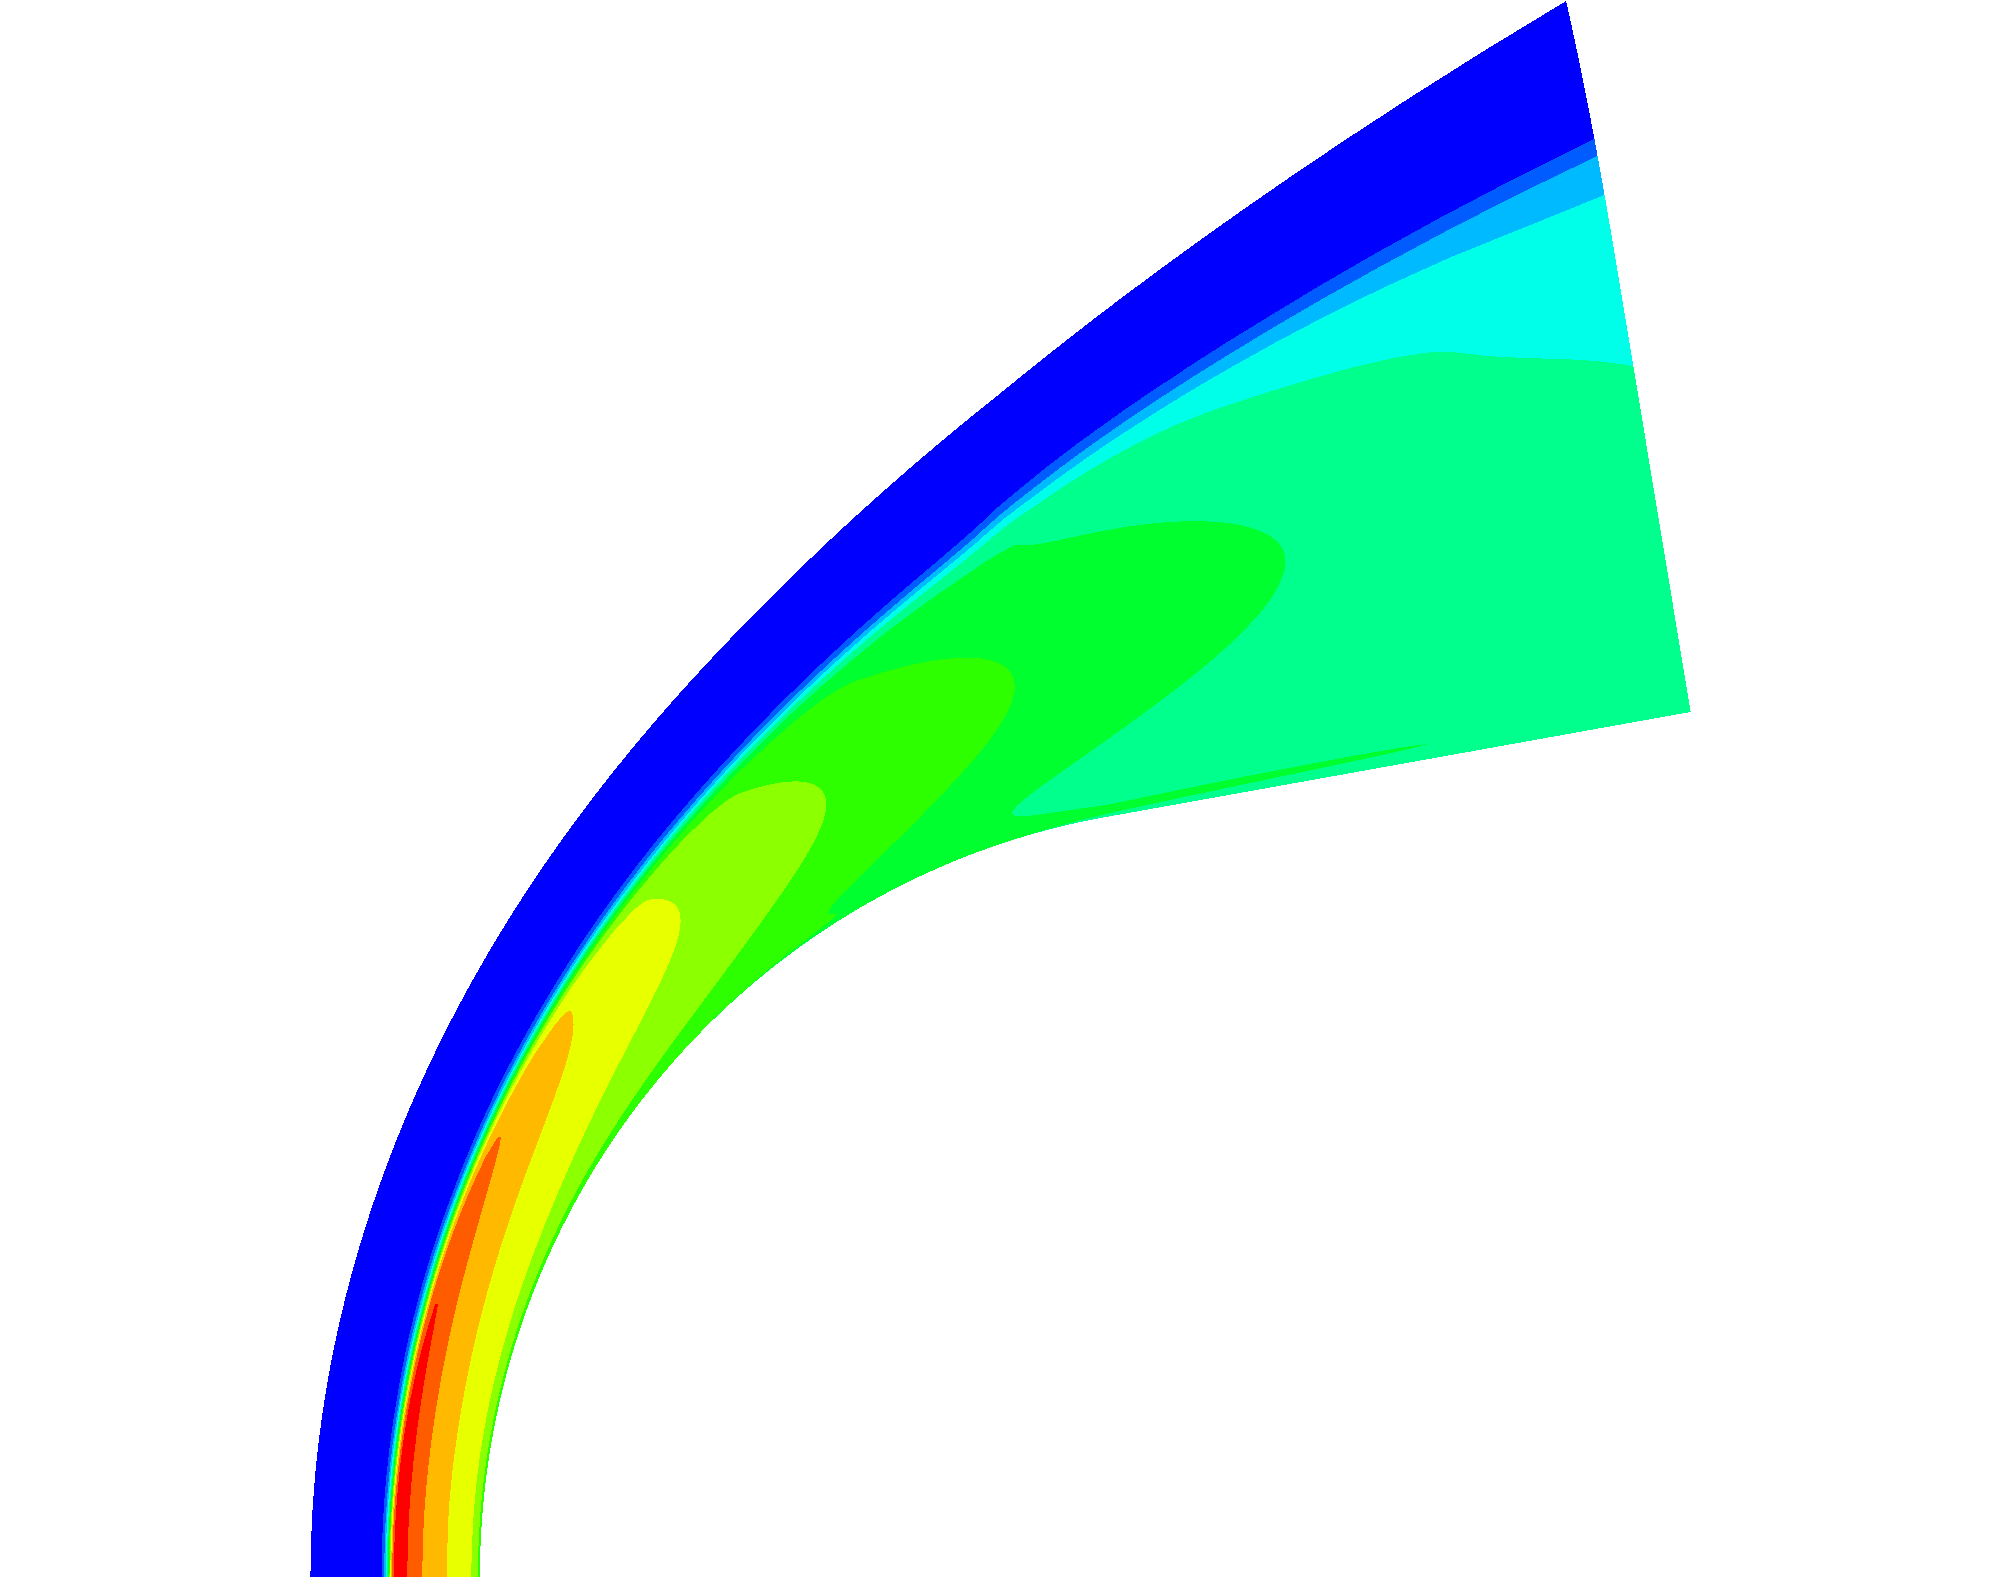
\includegraphics[height=\linewidth]{nosetip/smeared.png}}
        \only<2>{\includegraphics[height=\linewidth]{nosetip/amr.png}}
        \only<3>{\includegraphics[height=\linewidth]{nosetip/smeared.pdf}}
        \only<4>{\includegraphics[height=\linewidth]{nosetip/amr.pdf}}
        \only<5>{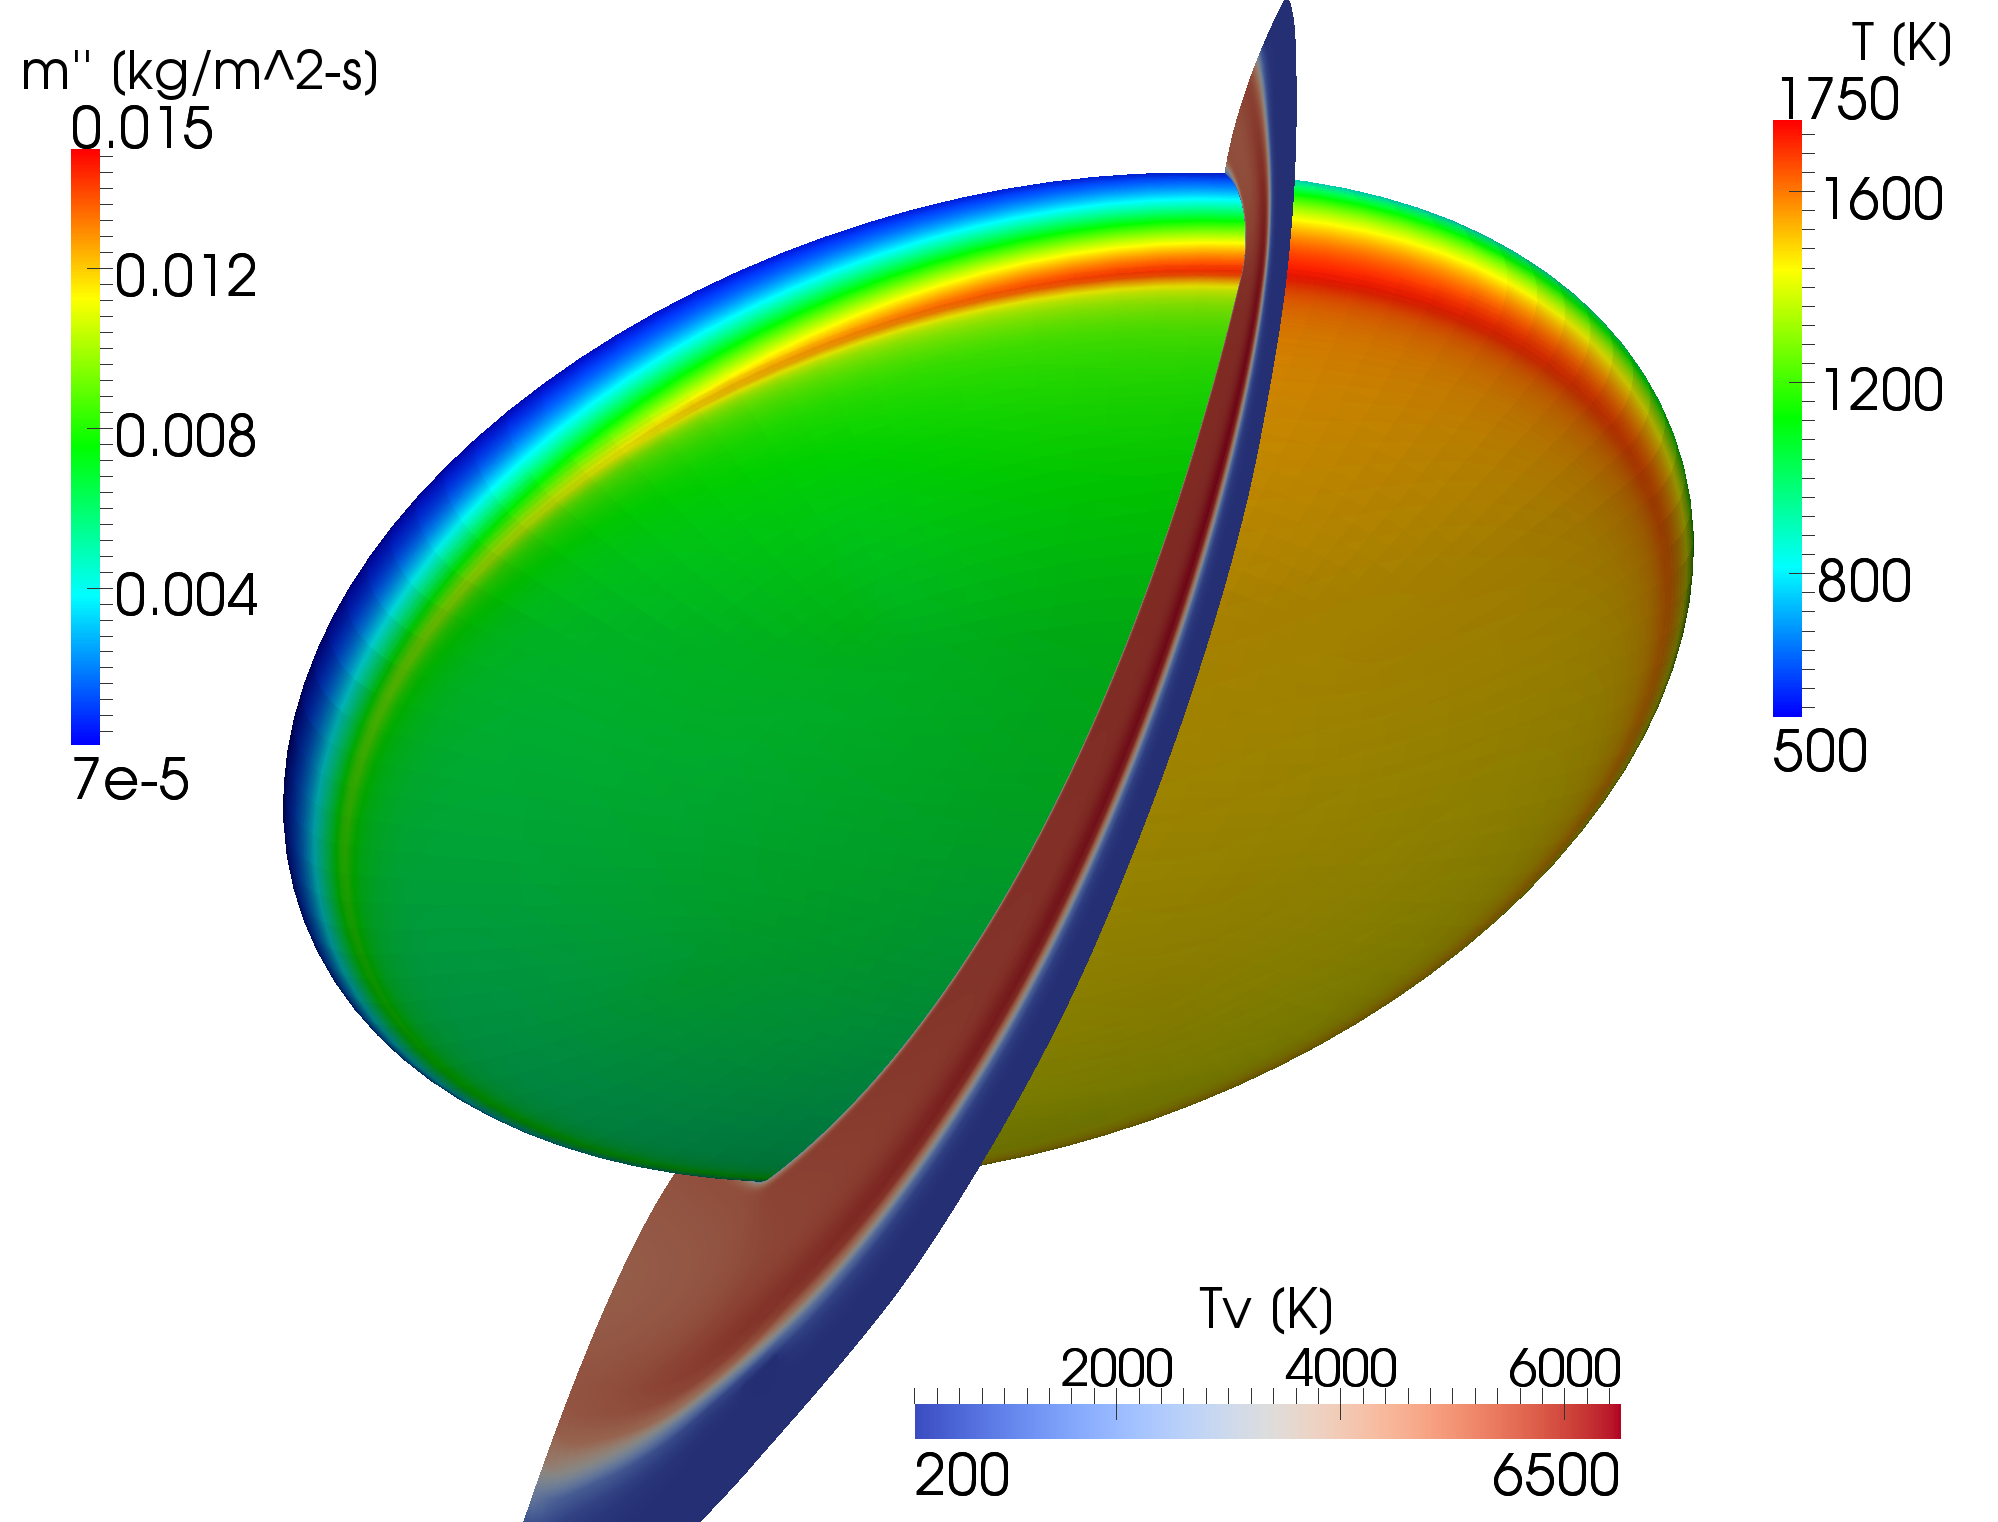
\includegraphics[height=\linewidth]{ablating_hs_wbg}}
      \end{center}
    \end{column}
  \end{columns}
}
%===============================================================================
% NEW SLIDE
%===============================================================================
\frame
{
  \frametitle{FIN-S: Arcjet Nozzle Calculation}
  \begin{center}
      
    \only<1>{\includegraphics[width=0.95\linewidth,trim=4px 4px 4px 4px,clip]{arcjet/viz/T}}
    
    \only<2>{\includegraphics[width=0.95\linewidth,trim=4px 4px 4px 4px,clip]{arcjet/viz/M}}
    
  \end{center}
}



%===============================================================================
% NEW SLIDE
%===============================================================================
%% \frame
%% {
%%   \frametitle{Arcjet Nozzle Calculation}
%%   \begin{center}

%%     \only<1>{\includegraphics[width=.95\textwidth,trim=4px 4px 4px 4px,clip]{arcjet/data/nozzle/P-streamlines.png}}

%%     \only<2>{\includemovie[autoplay,loop,text={\includegraphics[width=.95\textwidth,trim=4px 4px 4px 4px,clip]{arcjet/data/nozzle/P-streamlines.png}}]{.95\textwidth}{}{rawfigs/arcjet/data/nozzle/P.avi}}

%%   \end{center}
%% }



%===============================================================================
% NEW SLIDE
%===============================================================================
%% \frame
%% {
%%   \frametitle{Coupled Pyrolysis, Temperature}
%%   \begin{center}

%%     \only<1>{\includegraphics[height=.85\textheight]{arcjet/data/coupled/T.png}}

%%     \only<2>{\includemovie[autoplay,loop,text={\includegraphics[height=.85\textheight]{arcjet/data/coupled/T.png}}]{}{.85\textheight}{rawfigs/arcjet/data/coupled/T.avi}}

%%   \end{center}
%% }


%===============================================================================
% NEW SLIDE
%===============================================================================
%% \frame
%% {
%%   \frametitle{Coupled Pyrolysis, Pyrolysis gas mass flux, $\dot{m}$}
%%   \begin{center}

%%     \only<1>{\includegraphics[height=.85\textheight]{arcjet/data/coupled/mdotzoom.png}}

%%     \only<2>{\includemovie[autoplay,loop,text={\includegraphics[height=.85\textheight]{arcjet/data/coupled/mdotzoom.png}}]{}{.85\textheight}{rawfigs/arcjet/data/coupled/mdotzoom.avi}}

%%   \end{center}
%% }



%% \frame
%% {
%%   \frametitle{The MOOSE Framework - Gaston et al., INL}
%%   \begin{center}
%%     \fbox{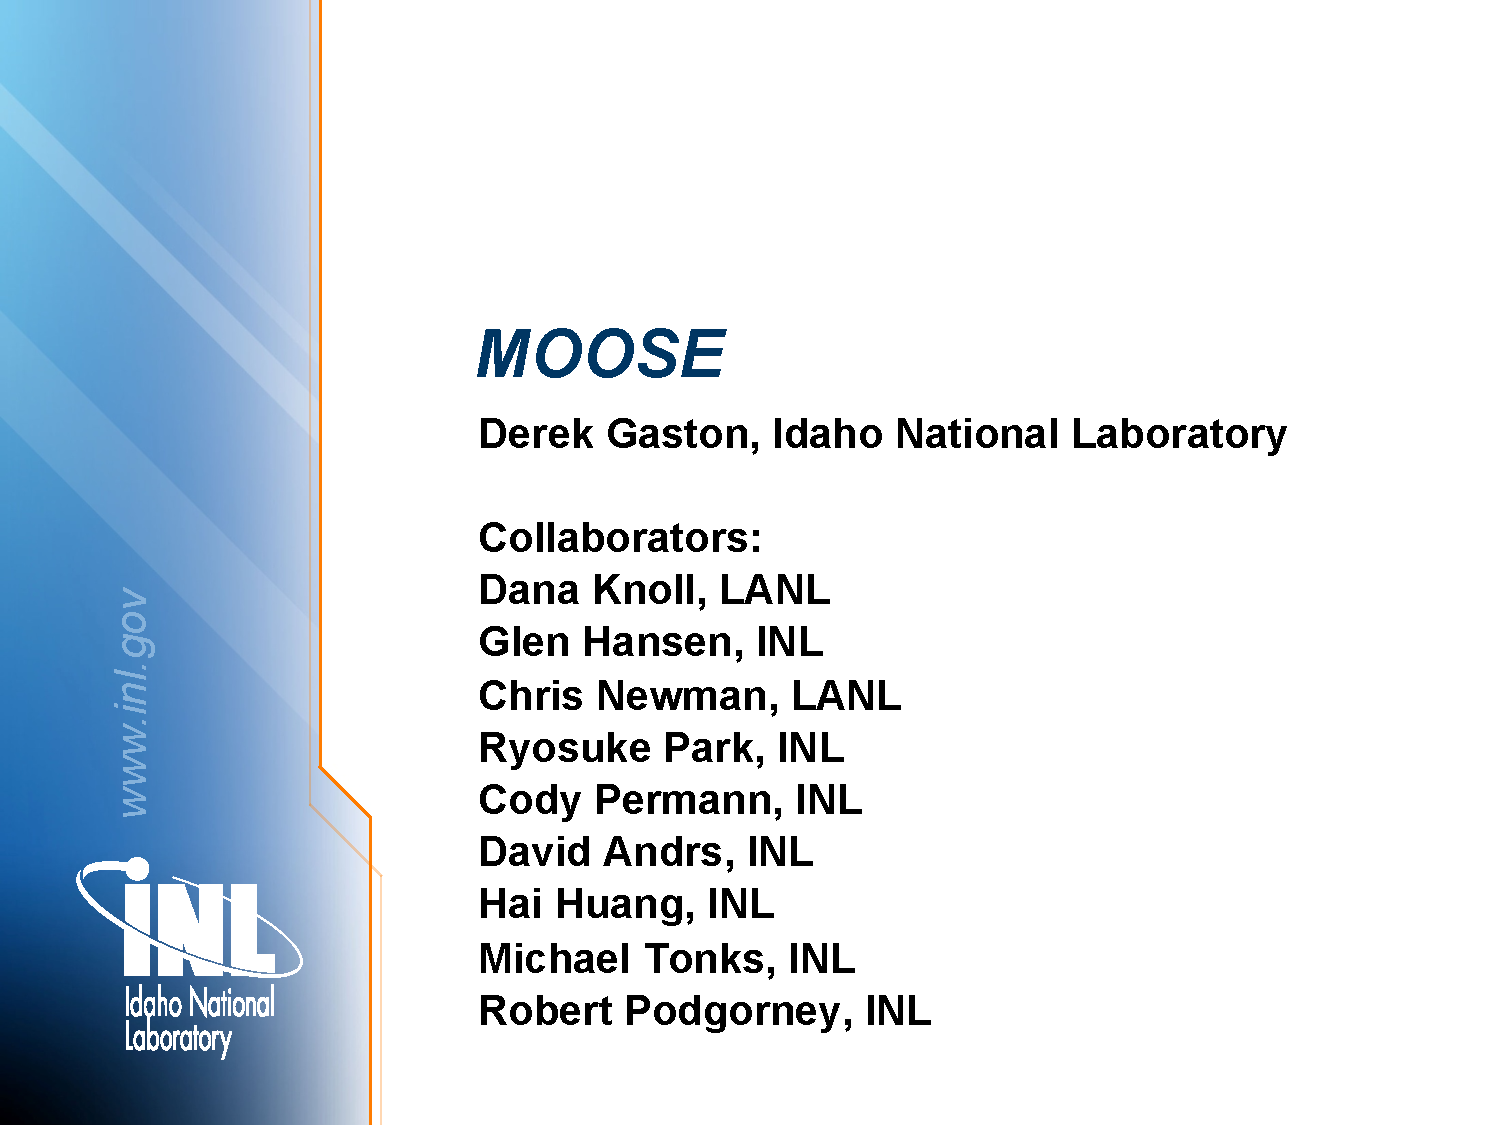
\includegraphics[page=1,height=0.8\textheight]{Gaston/talk}}
%%   \end{center}
%% }



\frame
{
  \frametitle{The MOOSE Framework - Gaston et al., INL}
  \begin{center}
    \fbox{\includegraphics[page=2,height=0.8\textheight]{Gaston/talk}}
  \end{center}
}



%% \frame
%% {
%%   \frametitle{The MOOSE Framework - Gaston et al., INL}
%%   \begin{center}
%%     \fbox{\includegraphics[page=4,height=0.8\textheight]{Gaston/talk}}
%%   \end{center}
%% }



\frame
{
  \frametitle{The MOOSE Framework - Gaston et al., INL}
  \begin{center}
    \fbox{\includegraphics[page=22,height=0.8\textheight]{Gaston/talk}}
  \end{center}
}

\frame
{
  \frametitle{Coupled Thermal/Solid Mechanics}
  \begin{center}

    \only<1>{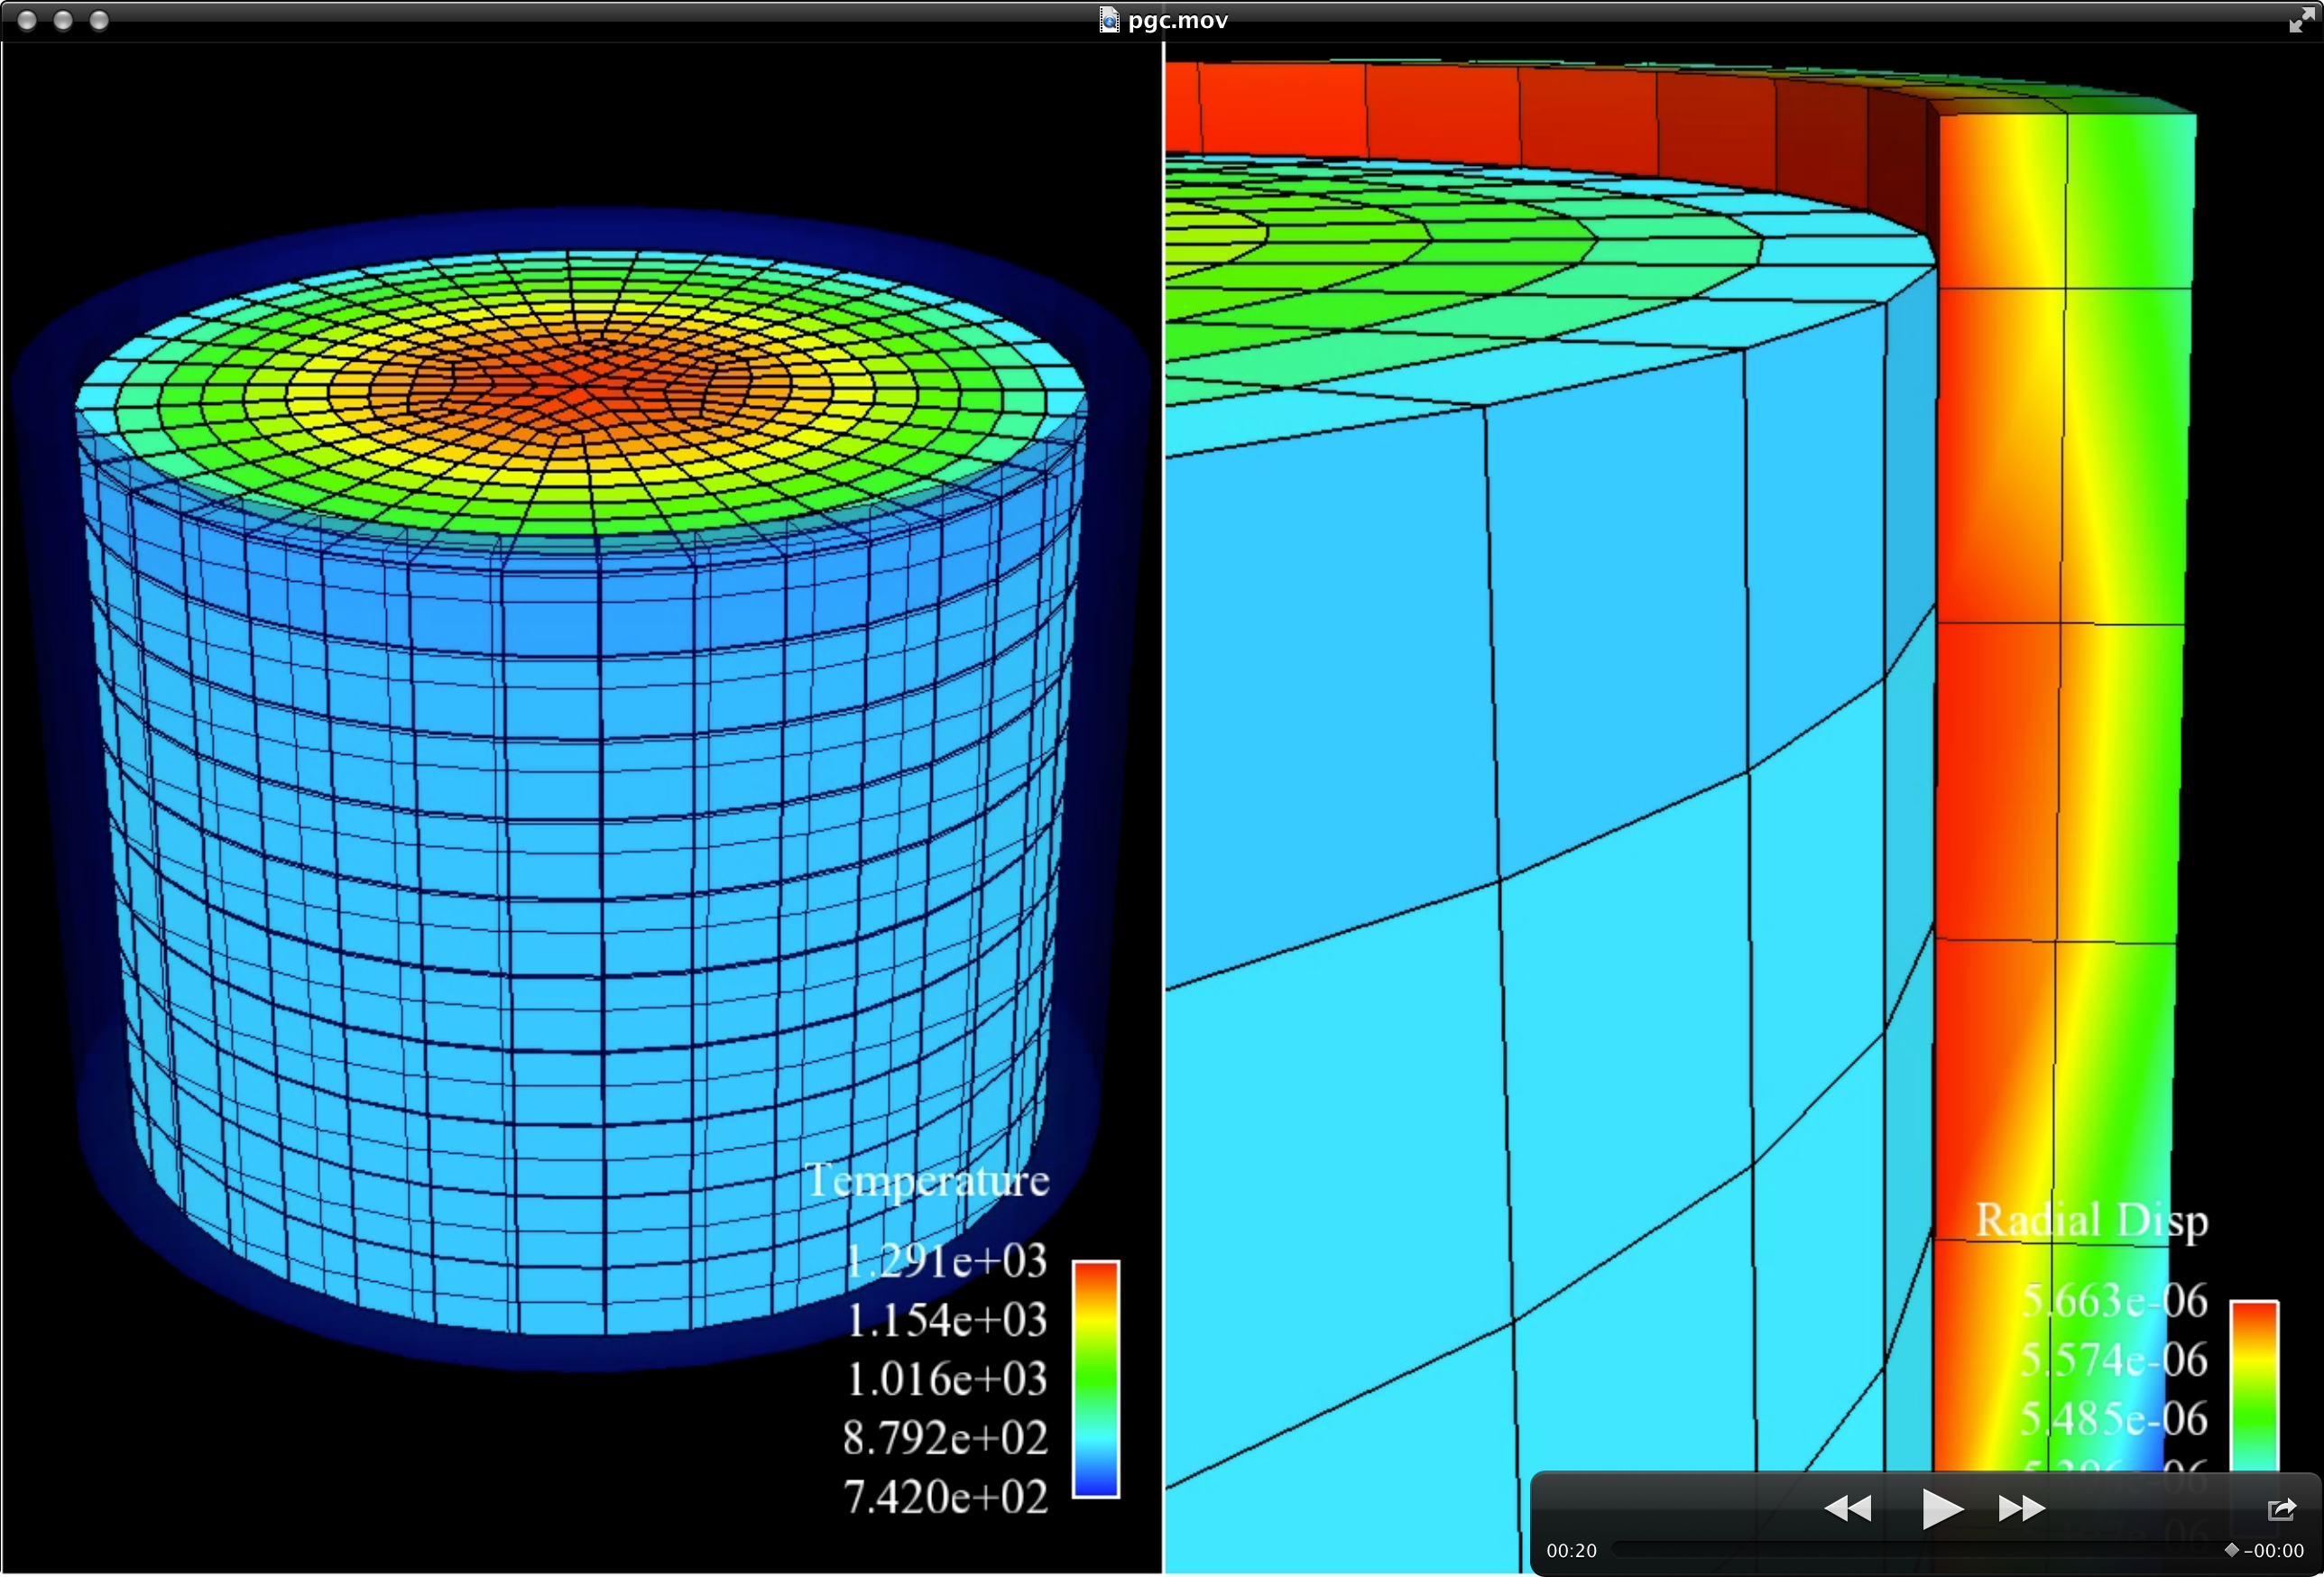
\includegraphics[height=.85\textheight]{Gaston/pgc.png}}

    \only<2>{\includemovie[autoplay,loop,text={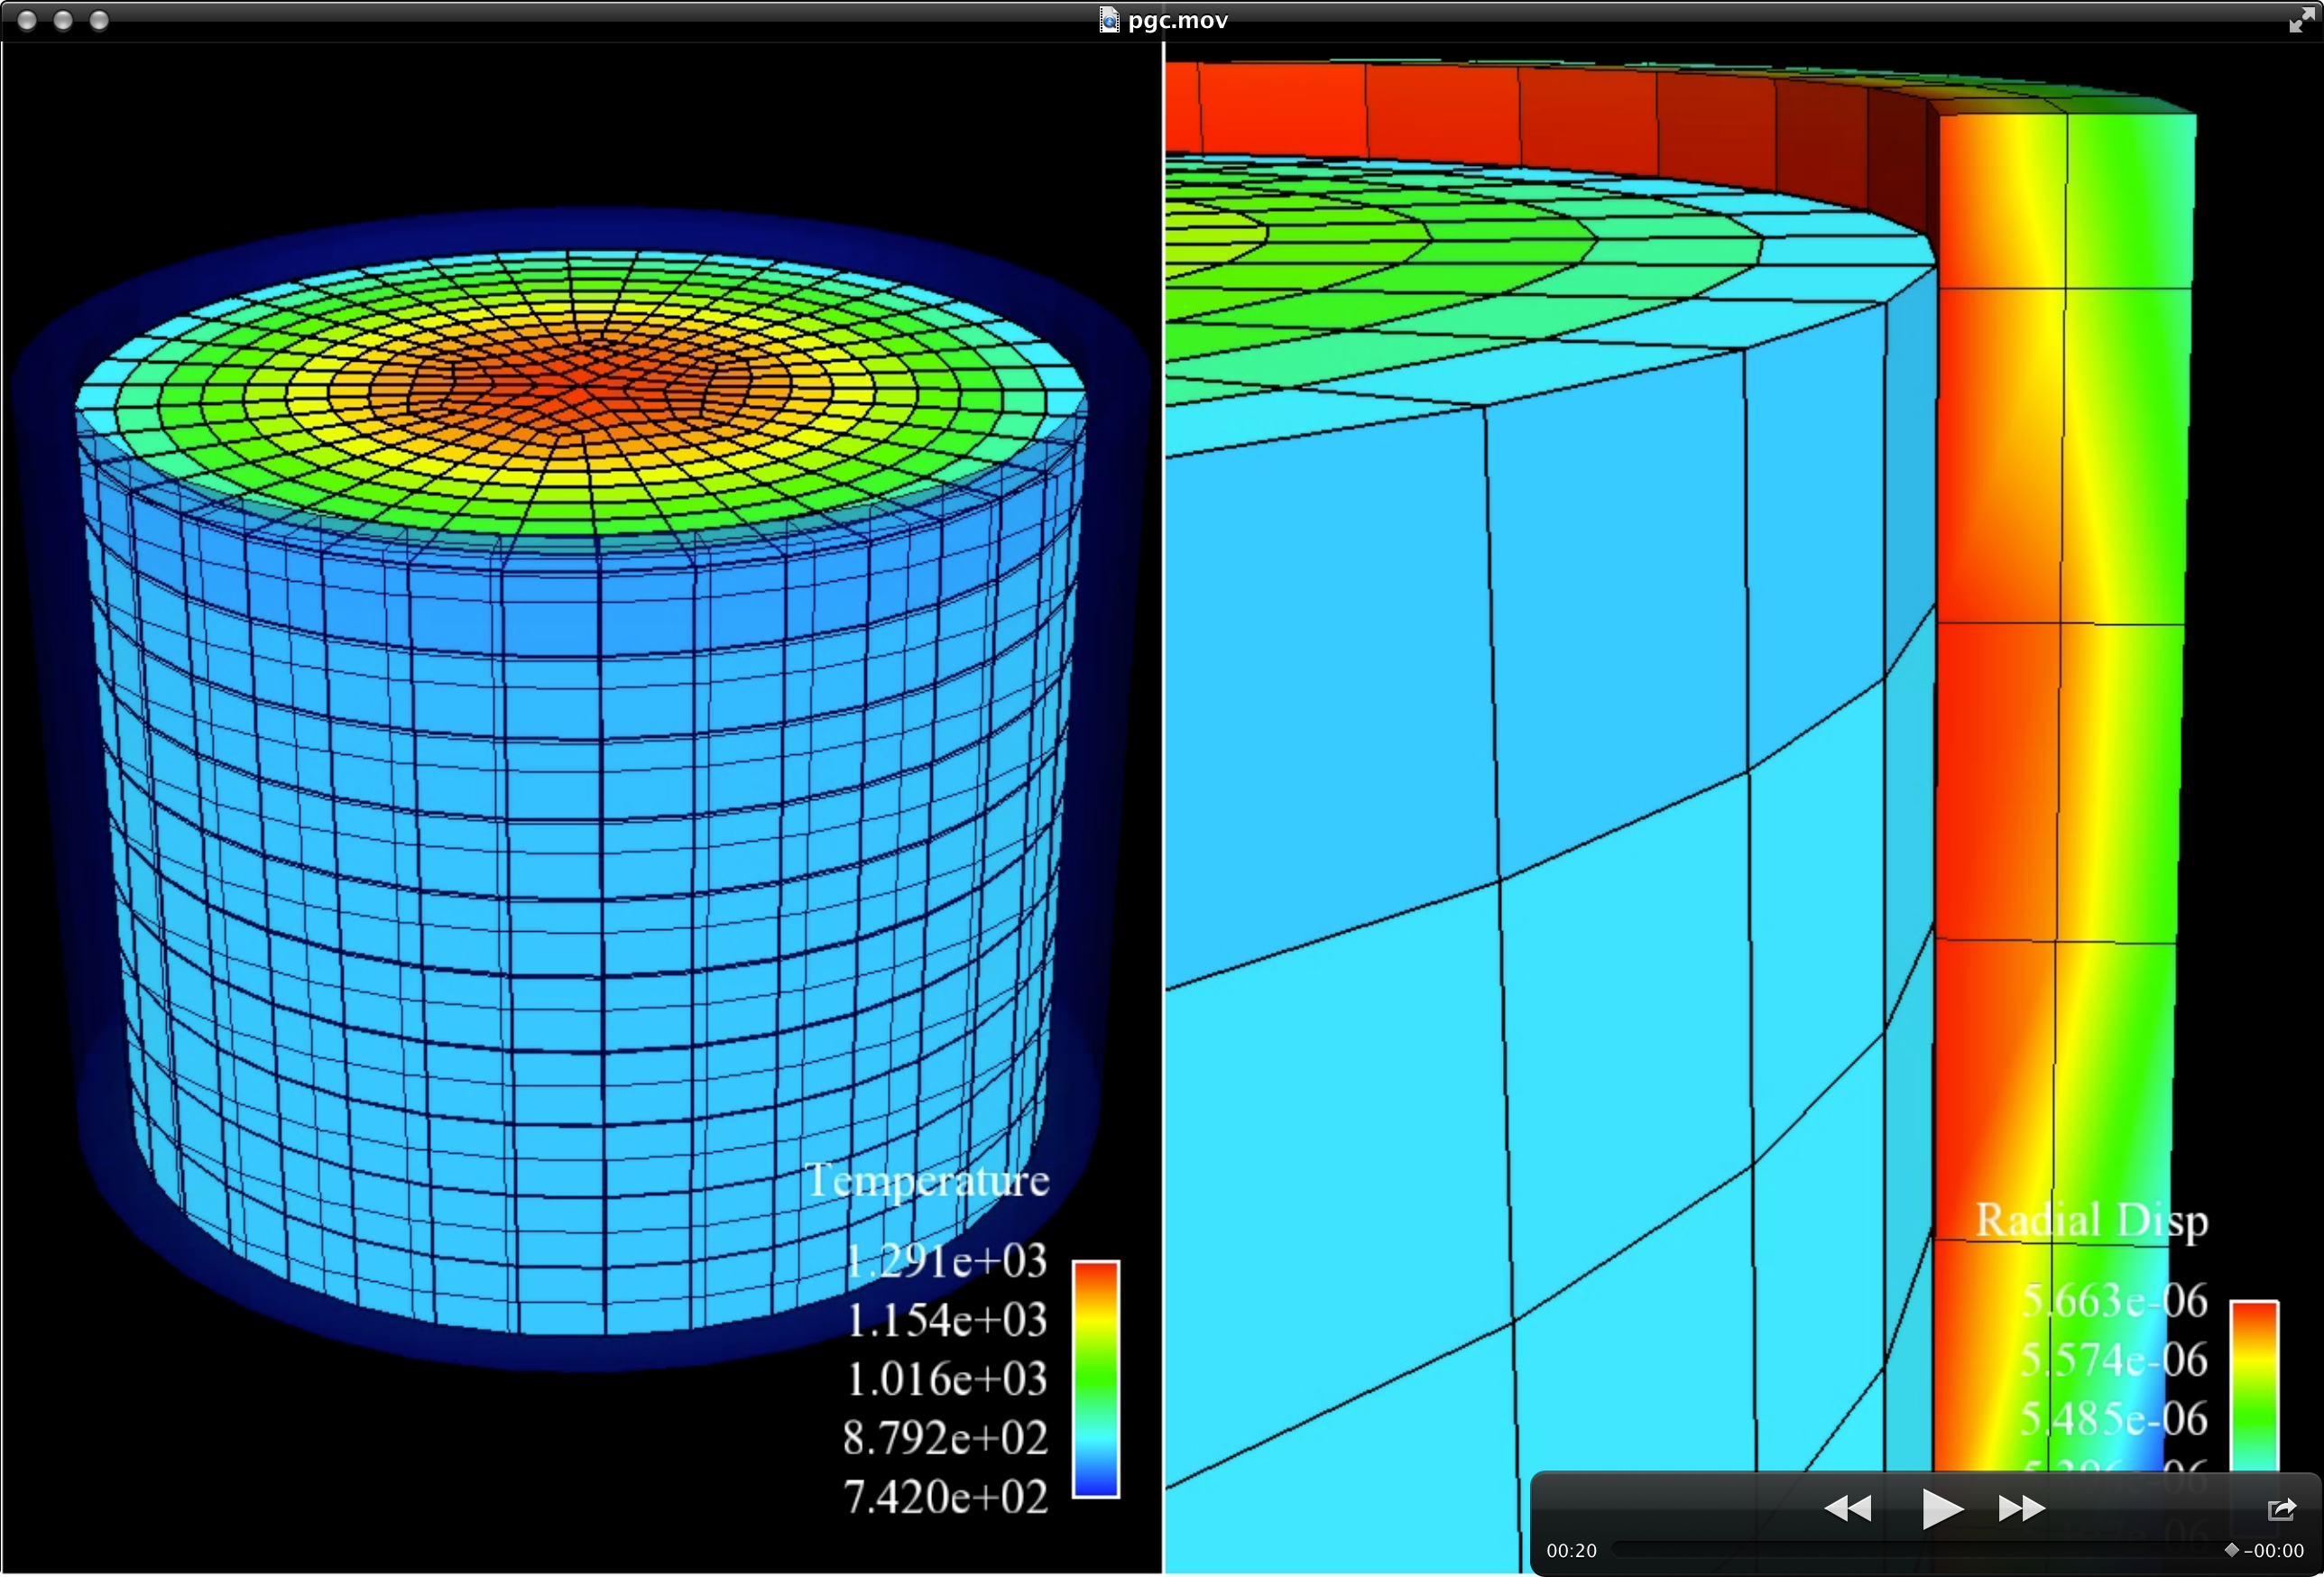
\includegraphics[height=.85\textheight]{Gaston/pgc.png}}]{}{.85\textheight}{Gaston/pgc.avi}}

  \end{center}
}


%===============================================================================
% New Slide
%===============================================================================
\begin{frame}
\frametitle{\texttt{GRINS}}

\begin{block}{\url{https://github.com/grinsfem/grins}}
  \begin{itemize}
  \item Multiphysics FEM platform built on \texttt{libMesh}
  \item Modular structure for ``Physics'', solvers, QoIs, etc.
  \item Key feature: automatically enabled discrete adjoints (AMR, sensitivities)
  \end{itemize}
\end{block}

\begin{columns}[T]
  \begin{column}{0.4\textwidth}
    \uncover<2->{\centerline{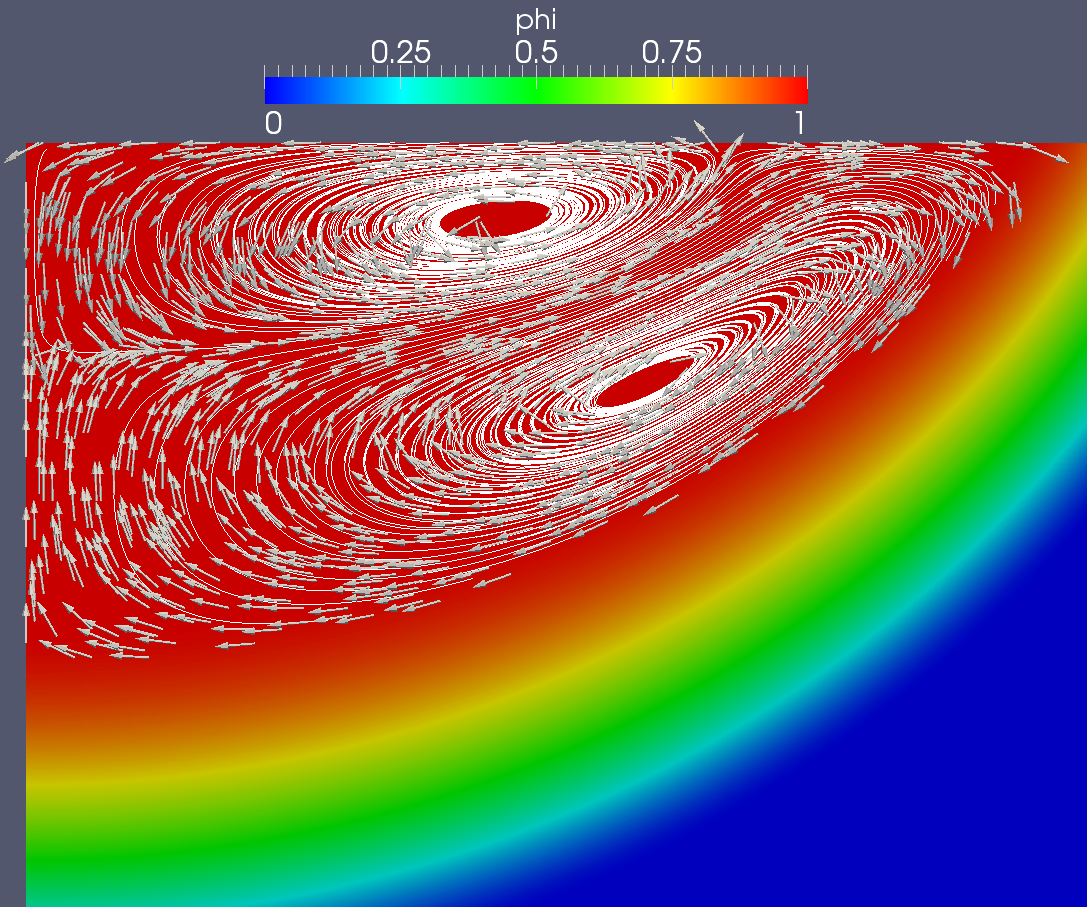
\includegraphics[width=\linewidth]{var_vortices}}}
  \end{column}
  %
  \begin{column}{0.4\textwidth}
    \only<3>{\centerline{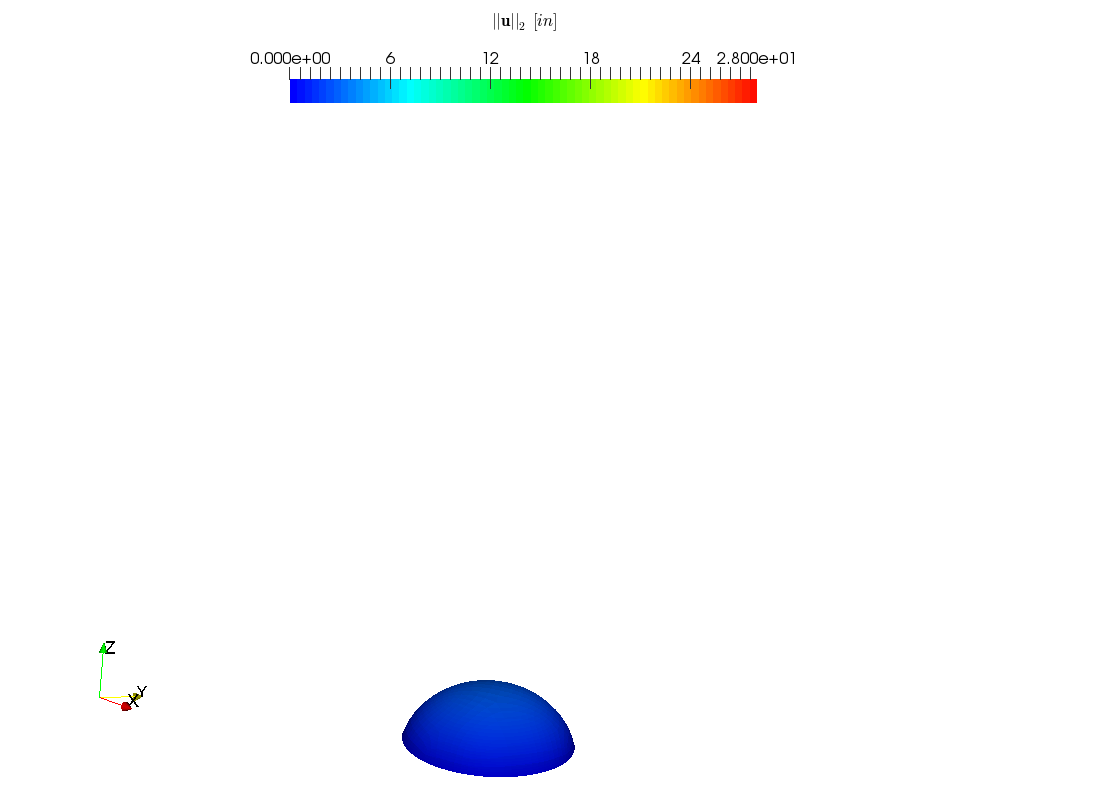
\includegraphics[width=\linewidth]{balloon_1}}}
    \uncover<4->{\centerline{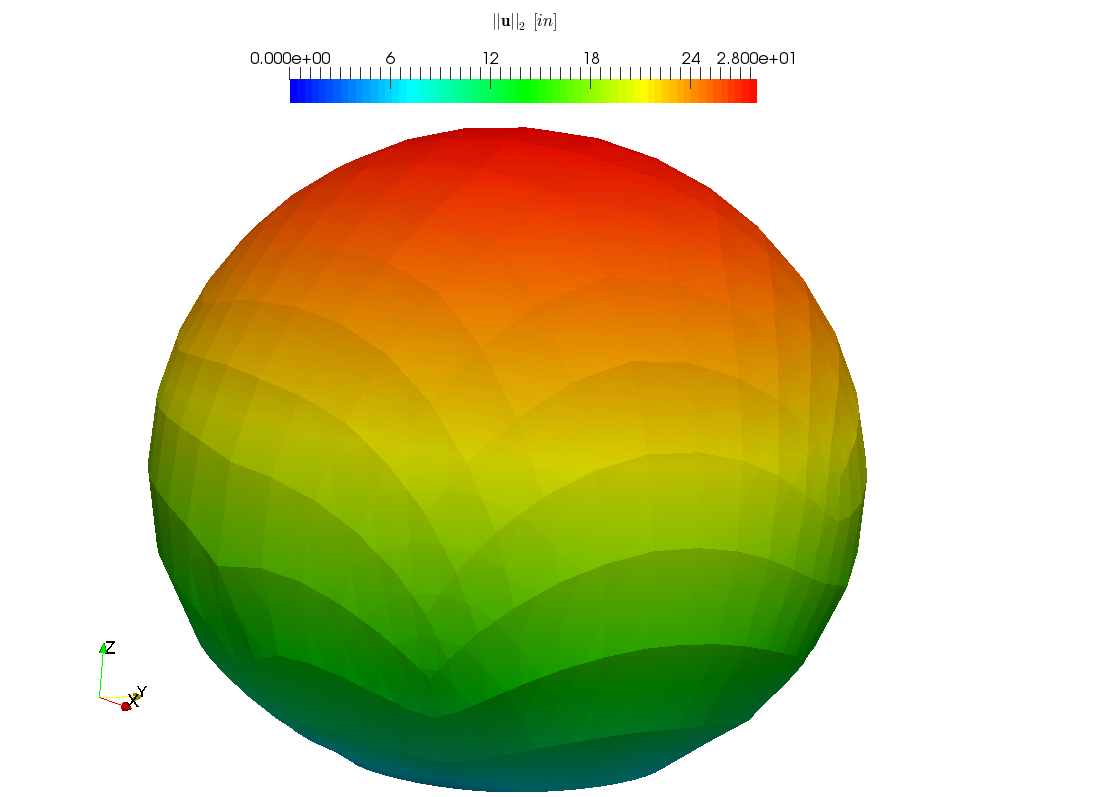
\includegraphics[width=\linewidth]{balloon_4}}}
  \end{column}
  %
  \begin{column}{0.2\textwidth}
    \uncover<5->{\centerline{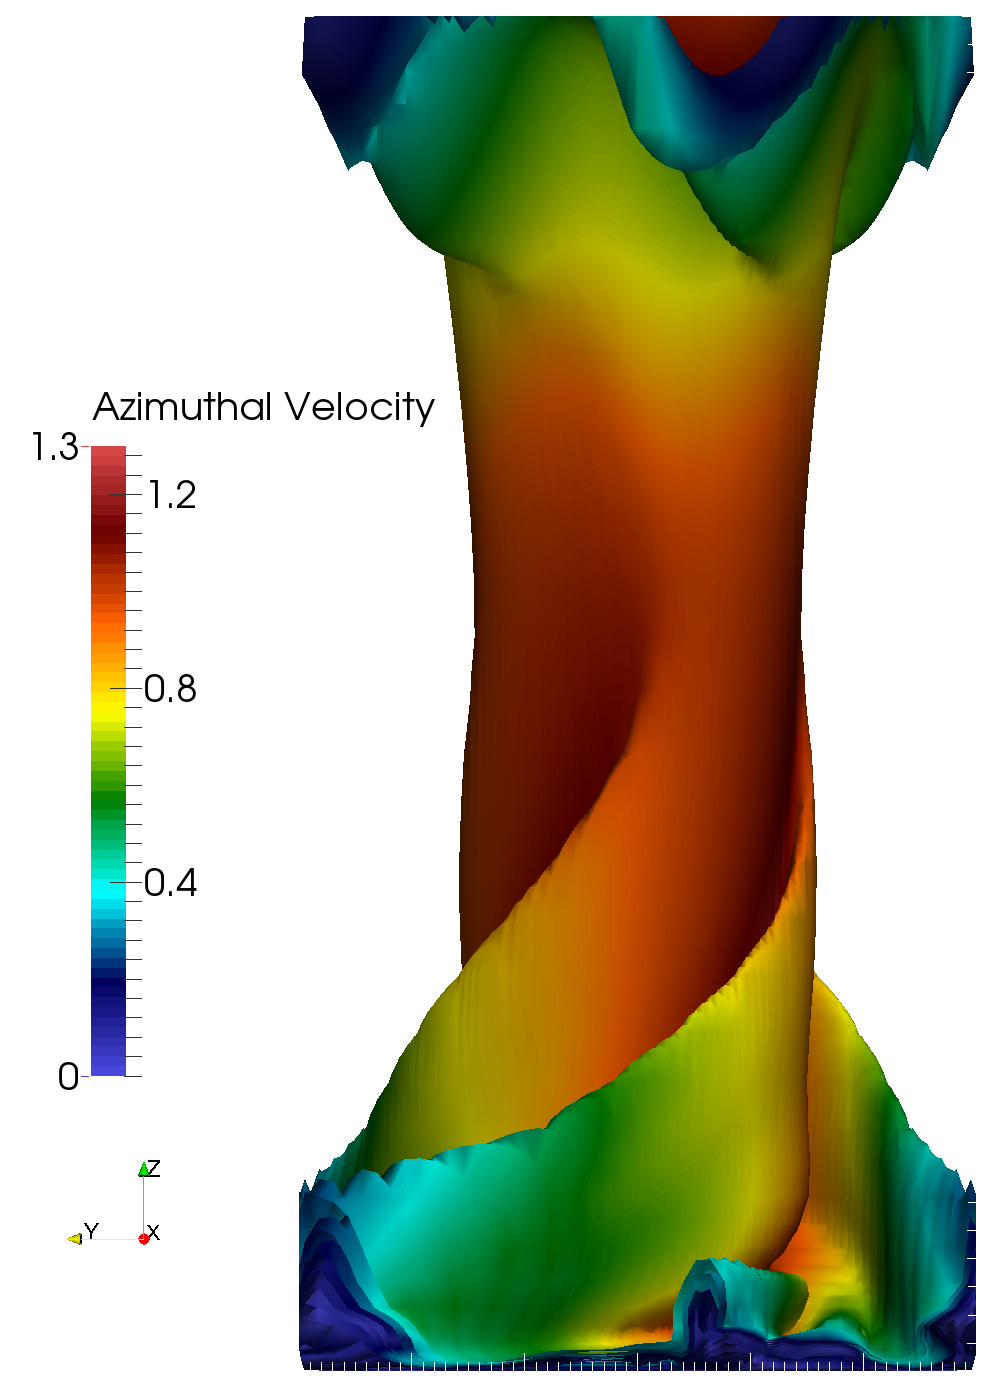
\includegraphics[width=\linewidth]{sov}}
    \tiny{Courtesy Nick Malaya, UT Austin}}
  \end{column}
  \end{columns}

\end{frame}

%===============================================================================
% New Slide
%===============================================================================
\begin{frame}
  \frametitle{\texttt{GRINS}}

\begin{block}{Ozone Flame}
  \only<1>{\centerline{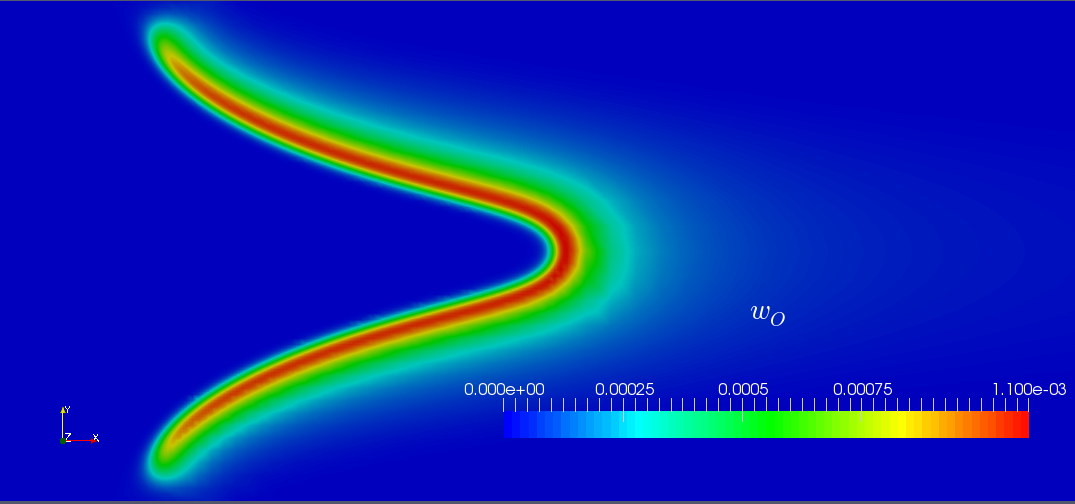
\includegraphics[width=0.9\linewidth]{ozone_flame_wo_nomesh}}}
  \only<2>{\centerline{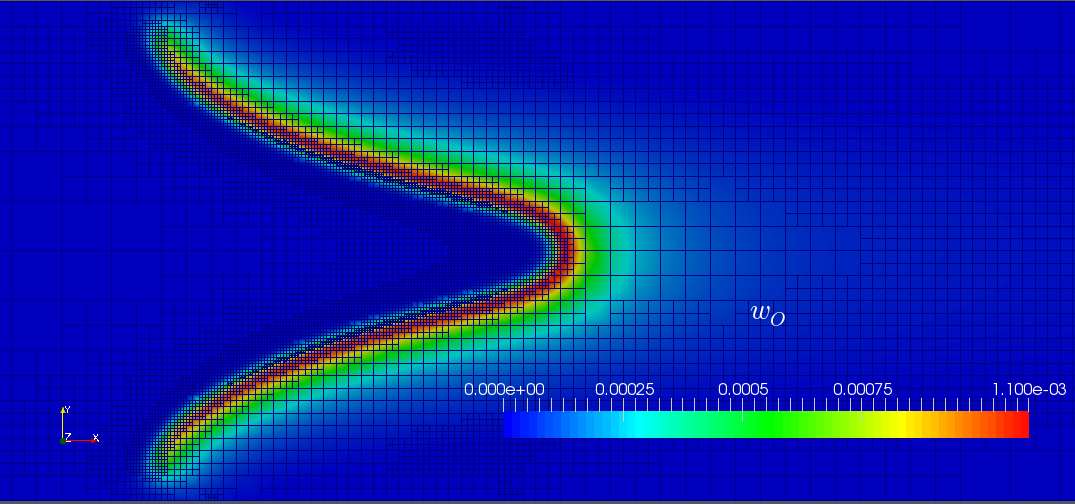
\includegraphics[width=0.9\linewidth]{ozone_flame_wo}}}
\end{block}


\end{frame}
